\section{Suma de enteros en base uno}

%----------
% MT-1A
%----------

\subsection{MT Determinista de 1 cinta}

\subsubsection*{Diseño propuesto}
El algoritmo de resolución es el siguiente:

\begin{itemize}
    \item Ciclo:
    \begin{enumerate}[1.]
        \item Desplazarse hasta el extremo derecho.
        \item Si el elmento es un 1:
        \begin{enumerate}[1.]
            \item Borrarlo.
            \item Volver al extremo izquierdo.
            \item Añadir un 1 en la primera posición.
        \end{enumerate}
        \item Si el elemnto es un \$:
        \begin{enumerate}[1.]
            \item Borrarlo.
            \item Volver al extremo izquierdo.
            \item \textbf{Parar}.
        \end{enumerate}
    \end{enumerate}
\end{itemize}

El diseño de la máquina queda representado en la Figura \ref{fig:MT-1A}.

\begin{figure}[h]
    \centering
    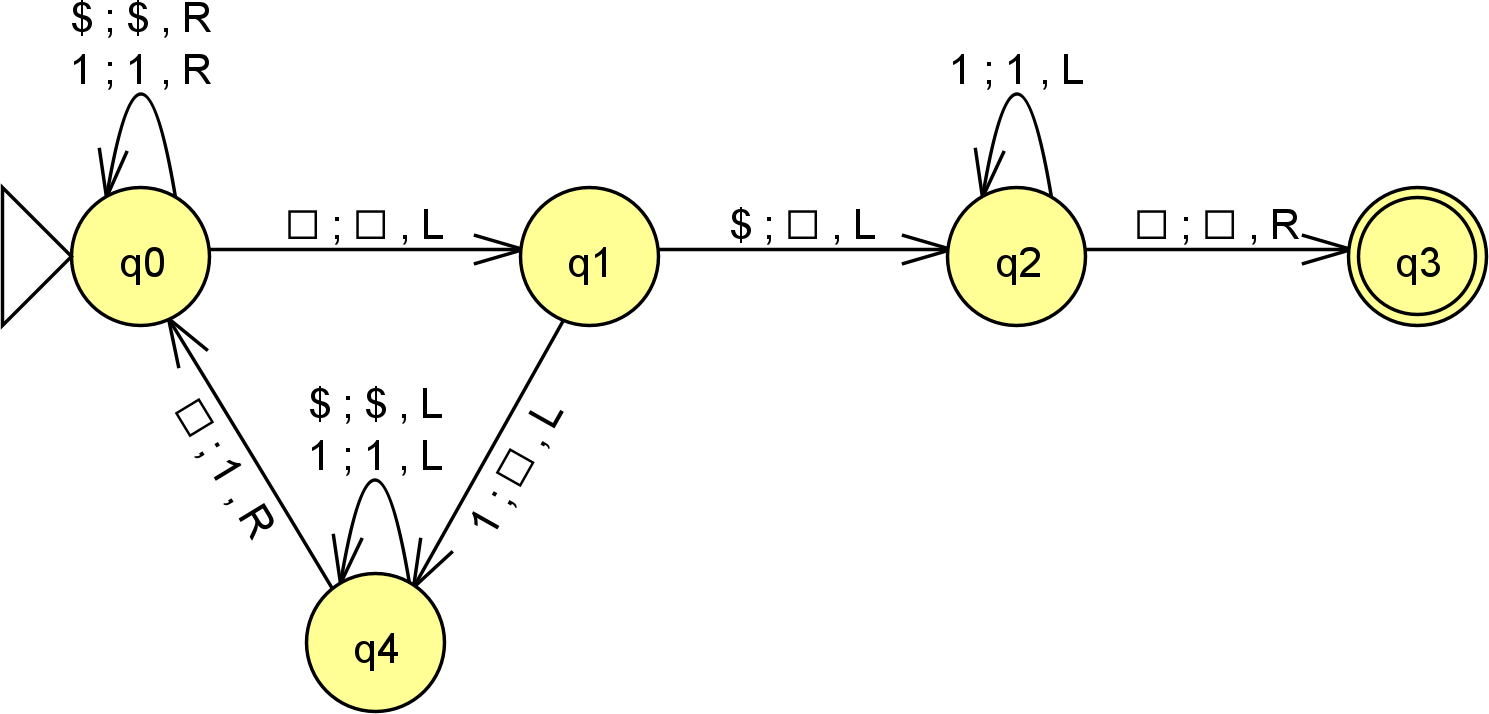
\includegraphics[width=0.6\textwidth]{MT-1A.png}
    \caption{Implementación en JFLAP de MT-1A}
    \label{fig:MT-1A}
\end{figure}


\subsubsection*{Peor caso}
Dado que el formato de palabra que acepta la Máquina de Turing son dos conjuntos de 1 separados por el simbolo \$, el peor caso sería aquel en el que haya una mayor cantidad de 1 a la derecha del \$, ya que por cada 1 se requerirá una iteración para eliminarlo de la derecha y añadirlo en la izquierda, por lo que a más 1 más iteraciones serán necesarias.

\subsubsection*{Evaluación empírica}
Realizamos la evaluación empírica en el peor caso, tomando como $n$ el número de 1 a la derecha de \$, ya que se trataría del peor caso, y midiendo el número de pasos realizados para resolver el problema\footnote{Los datos se pueden encontrar en \texttt{data/MT-1A.csv}.}:

\begin{table}[h]
    \centering
    \begin{tabular}{lcc}
        Entrada                & $n$ & Pasos \\
        \hline
        $\lambda$               & 0  & N/A \\
        \$1                     & 1  & 11  \\
        \$11                    & 2  & 22  \\
        \$111                   & 3  & 37  \\
        \$1111                  & 4  & 56  \\
        \$11111                 & 5  & 79  \\
    \end{tabular}
\end{table}


\subsubsection*{Coste computacional}
Para obtener el coste computacional del algoritmo, aplicaremos Diferencias Finitas, basándonos en los datos de la evaluación empírica:

\begin{table}[h]
    \centering
    \begin{tabular}{|l|c|c|c|c|c|}
        \hline
        $n$ & \textbf{1} & \textbf{2} & \textbf{3} & \textbf{4} & \textbf{5}\\ \hline
        $T(n)$ & \textbf{11} & \textbf{22} & \textbf{37} & \textbf{56} & \textbf{79}      \\ \hline
        \hline
        $A(n) = T(n) - T(n-2)$ &    & 11 & 15 & 19 & 23\\ \hline
        $B(n) = A(n) - A(n-2)$ &    &    &  4 &  4 &  4\\ \hline
        $C(n) = B(n) - B(n-2)$ &    &    &    &  0 &  0 \\ \hline
    \end{tabular}
\end{table}

Se obsrerva que las diferencias finitas segundas son constantes y nulas las terceras, por lo que podemos aproximar $T(n)$ con un polinomio de segundo orden, es decir, $T(n) = an^2 + bn + c$.\\

Para obtener los valores de $a$, $b$, y $c$, usaremos valores de $n$ y $T(n)$ obtenidos en la evaluación empírica:

\begin{subequations}
    \begin{gather}
        n = 1,\ T(1) = 11 \rightarrow a + b + c = 11 \\
        n = 2,\ T(2) = 15 \rightarrow 4a + 2b + c = 15 \\
        n = 3,\ T(3) = 19 \rightarrow 9a + 3b + c = 19
    \end{gather}
\end{subequations}

Resolviendo, $a=0$, $b=4$ y $b=7$, por lo que:

\begin{equation}
    T_{\mathrm{1A}}(n) = 4n + 7
\end{equation}

\subsubsection*{Cota asintótica}
Al conocer $T_{\mathrm{1A}}(n)$, podemos afirmar que $g(n) = n$. Si asumimos $n_0 = 10$, obtenemos $k \geq \frac{47}{10}$, por lo que la cota asintótica (definida en la ecuación \ref{eq:On}) para esta máquina es:
\begin{equation}
    T_{\mathrm{1A}}(n) = \frac{47}{10} n
\end{equation}


%----------
% MT-1B
%----------

\subsection{MT Determinista de 2 cintas}

\subsubsection*{Diseño propuesto}
El algoritmo de resolución es el siguiente:

\begin{itemize}
    \item Ciclo:
    \begin{enumerate}[1.]
        \item Comenzar desde la izquierda en ambas cintas e ir desplazandose hasta el extremo derecho.
        \item Si se encuentra un 1 en la cinta 0:
        \begin{enumerate}[1.]
            \item Borrarlo de la cinta 0.
            \item Añadir un 1 en la cinta 1.
        \end{enumerate}
        \item Si se encuentra un \$ en la cinta 0:
        \begin{enumerate}[1.]
            \item Borrarlo de la cinta 0.
            \item No añadir nada en la cinta 1 y no avanzar en dicha cinta
        \end{enumerate}
        \item Cuando se llega al final de la cinta 0, \textbf{parar}.
    \end{enumerate}
\end{itemize}
De esta forma la primera cinta quedaría vacía y la solución resultante de la suma quedaría en la segunda cinta\\

El diseño de la máquina queda representado en la Figura \ref{fig:MT-1B}.

\begin{figure}[h]
    \centering
    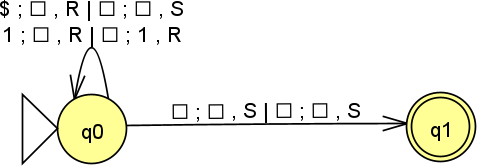
\includegraphics[width=0.5\textwidth]{MT-1B.png}
    \caption{Implementación en JFLAP de MT-1B}
    \label{fig:MT-1B}
\end{figure}


\subsubsection*{Peor caso}
En este algoritmo, el peor caso es independiente de si es mayor el número de la derecha que el de la izquierda, puesto que realiza el mismo recorrido, sin embargo el hecho de que haya números en ambos lados le añade un paso extra frente al hecho de que solo los haya en uno de los dos.


\subsubsection*{Evaluación empírica}
Realizamos la evaluación empírica en el peor caso, tomando como $n$ la longitud de la cadena de entrada.\footnote{Los datos se pueden encontrar en \texttt{data/MT-1A.csv}.}:

\begin{table}[h]
    \centering
    \begin{tabular}{lcc}
        Entrada                    & $n$ & Pasos \\
        \hline
        1\$1                       & 3  &  4  \\
        1\$11                      & 4  &  5  \\
        1\$111                     & 5  &  6  \\
        1\$1111                    & 6  &  7  \\
        1\$11111                   & 7  &  8  \\
    \end{tabular}
\end{table}


\subsubsection*{Coste computacional}
Para obtener el coste computacional del algoritmo, aplicaremos Diferencias Finitas, basándonos en los datos de la evaluación empírica:

\begin{table}[h]
    \centering
    \begin{tabular}{|l|c|c|c|c|c|c|c|}
        \hline
        $n$ & \textbf{3} & \textbf{4} & \textbf{5} & \textbf{6} & \textbf{7}\\ \hline
        $T(n)$ & \textbf{4} & \textbf{5} & \textbf{6} & \textbf{7} & \textbf{8}      \\ \hline
        \hline
        $A(n) = T(n) - T(n-2)$ &    & 1 & 1 & 1 & 1 \\ \hline
        $B(n) = A(n) - A(n-2)$ &    &   & 0 & 0 & 0 \\ \hline
    \end{tabular}
\end{table}

Se obsrerva que las diferencias finitas primeras son constantes y nulas las segundas, por lo que podemos aproximar $T(n)$ con un polinomio de primer orden, es decir, $T(n) = an + b$.\\

Para obtener los valores de $a$ y $b$, usaremos valores de $n$ y $T(n)$ obtenidos en la evaluación empírica:

\begin{subequations}
    \begin{gather}
        n = 3,\ T(3) = 4 \rightarrow 3a + b = 4 \\
        n = 4,\ T(4) = 5 \rightarrow 4a + b = 5 \\
    \end{gather}
\end{subequations}

Resolviendo, $a = b = 1$, por lo que:

\begin{equation}
    T_{\mathrm{1B}}(n) = n + 1
\end{equation}

\subsubsection*{Cota asintótica}
Al conocer $T_{\mathrm{1B}}(n)$, podemos afirmar que $g(n) = n$. Si asumimos $n_0 = 10$, obtenemos $k \geq \frac{11}{10}$, por lo que la cota asintótica (definida en la ecuación \ref{eq:On}) para esta máquina es:
\begin{equation}
    T_{\mathrm{1A}}(n) = \frac{11}{10} n
\end{equation}